\chapter{Понятие статистический анализ кода}

 \section{Что такое анализ кода}

Анализ -- один из методов исследования предметной области. Сущность метода заключается разделения большей сущности на меньшие для получения информации о структуре объекта исследования. Метод выделяет факты относящиеся непосредственно к предметной области или изучаемому объекту. Если рассматривать анализ относительно области программных продуктов, какими являются, например, программное обеспечение, то можно выделить в процессе работы метода совокупность программ, процедур, правил позволяющих выполнять деятельность описанную в документах по эксплуатации \cite{6}.

В случае анализа кода выделяются два метода для выполнения метода: динамический и статический анализ. 
 
Динамический анализ кода -- вид анализа, в процессе которого учувствуют программы использующие реальные или виртуальные процессоры. Инструменты динамического анализа, обычно, запрашивают установку и настройку специализированных библиотек для корректной работы, а так же возможность перекомпиляции программного кода. Существуют виды утилит позволяющие анализировать выполняемый код в ходе выполнения или же перед анализируемым блоком кода. Чтобы получить достаточную полезность от инструментов динамического анализа, ставится задача по набору достаточного количество входных данных, для анализа большего количества, в процентном соотношении, исходного кода. Одним из важных факторов, оказывающих на результаты анализа является влияние инструментов динамического анализа на эффективность выполнения анализируемого ПО. Такое воздействие, для получения более достоверных результатов, нужно свести к минимуму \cite{1}. 

В качестве инструментов в предметной области, связанной с программированием, воспринимаются те, что имеют возможность для отслеживания и установки количественных и качественных характеристик продукта, и выполняющие процессы по диагностике ошибок процесса выполнения и их причин возникновения с последующей записью информации для анализа группой тестирования. Для эффективного управления инструментами анализа в приложение временно встраивается код инструментов, управление которым, осуществляется при помощи внешних инструментов-утилит. Получаемые результаты измерений используются для последующей доработки программ, исправлению критических ситуаций, оптимизации и других потребностей по улучшению продукта. Из основных типов измерений выделяются проведение замеров на основе исходного кода программного продукта и его двоичной реализации \cite{2,3}. 

Статический анализатор кода -- это программа или совокупность различных модулей, направленных на проведение анализа кода изложенного в файле без выполнения кода в рабочей программе. В случае если компилятор находит ошибки или неточности синтаксического характера, то статический анализ позволяет глубоко погружаться в контекст написанного кода программистом, для тонкого понимания хода программы в том или ином блоке кода, а также отдельно и в совокупности проверяя возможность и результат работы написанных команд. 

Статический анализ кода относится к анализу семантики и поведения кода без фактического выполнения программы, тем самым выявляя семантику программы или неоднозначное поведение, которое является ненормальным из-за неправильного кодирования программы. С точки зрения непрофессионала, статический анализ кода заключается в выявлении ошибок кодирования кода одновременно с написанием кода. Тем самым не нужно ждать, пока будет написан весь код, и не нужно создавать рабочую среду, писать тестовые примеры. Он может обнаруживать различные проблемы в коде на ранних стадиях процесса разработки программного обеспечения, тем самым повышая эффективность разработки и качество программного обеспечения \cite{4,5}.


\section{Цели внедрения статического анализа в процесс разработки}

\begin{enumerate}

    \item Улавливание потенциальных ошибок. Одним из наиболее известных применений статического анализатора кода является поиск потенциальных проблем и дефектов в программном обеспечении. Эти проблемы варьируются от ошибочного не написания инструкции \verb|\break| переключения, до потенциального переполнения буфера, стека и проблем с памятью. Статический анализатор кода обладает способностью находить программные проблемы, которые обычно игнорируются компиляторами и инженерами, просматривающими код. Хорошей практикой является установка статического анализатора кода на ранней стадии реализации, чтобы гарантировать, что потенциальные проблемы будут устранены немедленно, а не позже в цикле разработки!

    \item недрение стандартов кодирования. Использование стандартов кодирования -- хороший способ гарантировать, что программное обеспечение разрабатывается согласованным и понятным образом. Стандарты кодирования не только определяют проблемы с удобочитаемостью, но и могут быть использованы для внедрения лучших практик. Хорошим примером стандарта кодирования, поддерживаемого многими статическими анализаторами кода, является MISRA Статический анализатор кода может использоваться для обеспечения того, чтобы разработчики встроенных систем не нарушали большинство рекомендаций или рекомендаций стандарта (однако некоторые правила требуют визуального осмотра, и соответствие не может быть определено автоматически). Если происходит нарушение, статический анализатор сообщит о нарушении разработчику и предпримет корректирующие действия. Результатом использования статического анализатора для выполнения стандартов кодирования является быстрое определение того, соответствует ли код определенным стандартам \cite{8,9}.
    
    \item Поддерживать строгое соответствие стандарту ANSI-C. Разработчики, которые заботятся о написании переносимого программного обеспечения, соответствующего стандарту ANSI-C, могут использовать статический анализатор, чтобы определить, используются ли какие-либо нестандартные языковые функции. Установка анализатора на уровень «строгий» определит области интересов, в которых переносимость на разные компиляторы или платформы может стать проблемой. Затем разработчики могут проверить эти области и улучшить программное обеспечение, чтобы оно лучше соответствовало стандарту ANSI-C, или, по крайней мере, записать, какие области программного обеспечения могут потребовать дополнительной работы по переносу \cite{10,11}.
    
    \item Выполнение строгой проверки типов.  Например, язык программирования C не поддерживает строгую проверку типов. В C, если разработчик хочет создать свой собственный тип, компилятор проигнорирует новый тип и вместо него будет использовать базовый тип C. Хороший анализатор способен воспринимать новый тип в контексте и использовать его как самостоятельную единицу в дальнейшем исследовании кода.
    
    \item Обеспечить смысловой контроль используемых переменных. Язык программирования C не может обеспечить какой-либо количественный анализ для обеспечения согласованности вычислений. Однако статический анализатор кода может выполнить эти проверки и убедиться, что расстояние случайно не умножается на футы и не дает неверных результатов. Настройки для количественного анализа варьируются от инструмента к инструменту, но это важная функция, которой разработчики должны воспользоваться \cite{7}.
    
    \item Поддержка базового анализа стека. Понимание разработчиками встраиваемых систем наихудшего использования стека имеет важное значение для разработки любой встраиваемой системы в реальном времени. Существует много способов проанализировать и определить наихудшее использование стека, но один из способов начать понимать использование стека — это использовать статический анализатор кода. Статический анализатор может вычислить диаграмму использования стека и вызова функции, чтобы получить общее представление о том, насколько глубоким должен быть стек. Инструменты статического анализатора также могут дать представление о том, как используются программные функции и считаются ли они детерминированными \cite{12}.
    
    \item Проверка ошибок многопоточных приложений и систем работы в реальном времени. Инструменты статического анализа также можно использовать для выявления проблем с потоками и задачами, выполняемыми на процессоре одновременно. Например, инструмент анализа может определить, существуют ли какие-либо исключения, связанные с блокировкой или разблокировкой мьютексов. Проверка потоков - очень полезный инструмент для выявления проблем в системах реального времени, но настройка такого рода анализа обычно не проста. Тем не менее, работа по настройке полезна для обнаружения неуловимых или аномальных событий потока \cite{13}.
    
\end{enumerate}


\section{Задачи, решаемые статическими анализаторов}

Статические анализаторы могут выполнять различные задачи, в зависимости от инструментальной наполненности и заданных настроек. На основе поставленных целей выделим общие задачи для статических анализаторов:

\begin{enumerate}

    \item Поиск ошибок в программном коде. Одна из самых часто решаемых задач для анализатора, в процессе поиска ошибок в коде по невнимательности, недостаточных знаний или иных проблем. Ошибки могут представлять собой от банальных опечаток в словах, до изменений на фундаментальном уровне работы с продуктом или библиотекой, о чем подскажет и направит анализатор;
    
    \item анализ кода как часть механизма Quality Gates в CI/CD. Анализаторы могут не только сообщать о наличии возможных ошибок в коде, но и служить защитным механизмом, предотвращающим доставку кода, если уровень его качества не соответствует заданным требованиям. Такую роль могут выполнять анализаторы кода, расширяющие поведение компилятора и блокирующие сборку, если были обнаружены ошибки или несоответствия кода принятым стандартам;
      
    \item улучшение качества кода в широком смысле этого слова. К качеству можно отнести читаемость, поддерживаемость и обновляемость, сложность кода, уровень связанности и другие аспекты, которые прямо или косвенно могут влиять на количество ошибок. Тем самым, статические анализаторы могут помогать следовать стандартам кодирования, которые могут быть созданы конкретной компанией для своих продуктов, так и общепринятым.
        
    \item сбор метрик проекта, сбор статистики, построение графиков и диаграмм, отражающих общее «состояние здоровья» проекта.  Метрика программного обеспечения -- это мера, позволяющая получить численное значение некоторого свойства программного обеспечения или его спецификаций.
          
\end{enumerate}

\section{Преимущества и недостатки внедрения инструментов статического анализа}

Многообразие инструментов статического анализа многократно уменьшает вероятность дорогих или, на позднем этапе, невозможных изменений для выпущенных устройств или ПО. 
Статический анализ не дает гарантию отсутствия ошибок в коде. Он выполняет функцию дополнительной возможности проверки корректности кода, программными средствами помимо человеческого ресурса. Инструменты выполняют свою работы много быстрее людей из-за чего стоимость затрат по времени столь несущественна по сравнению с результатами, которые они дают. В зависимости от используемого ПО для статического анализа меняется количество, качество и разнообразие типов ошибок, которые может обрабатывать и выдавать рекомендации анализатор \cite{14}.

Главное преимущество статического анализ состоит в возможности существенной снижении стоимости устранения дефектов в программе. Чем раньше ошибка выявлена, тем меньше стоимость ее исправления. Так согласно данным, приведенным в книге Макконнелла \guillemotleftСовершенный Код\guillemotright, исправление ошибки на этапе тестирования обойдется в десять раз дороже, чем на этапе конструирования (Рисунок \ref{fig:1}):


    \begin{figure}[!h]
    \center
    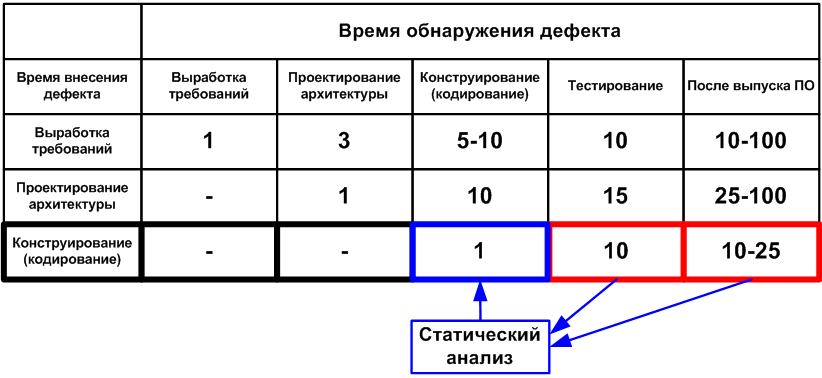
\includegraphics[width=15cm]{Images/Time to detect.png}
    \caption{Средняя стоимость исправления дефектов в зависимости от времени их внесения и обнаружения }
    \textwidth{ https://import.viva64.com/docx/terminology/Staticcodeanalysisru/image2.png}
        \label{fig:1}
    \end{figure}

Иные преимущества статического анализа кода:

\begin{enumerate}

    \item полное покрытие кода. Статические анализаторы проверяют даже те фрагменты кода, которые испоьзуются не часто, или были созданы очень давно. Такие участки кода, как правило, не удается протестировать другими методами или же тестирование проводилось ранее, а на данных момент считается излишним. Это позволяет находить дефекты в обработчиках редких ситуаций, в обработчиках ошибок или в системе логирования \cite{15};
    
    \item статический анализ не зависит от используемого компилятора и среды, в которой будет выполняться скомпилированная программа. Это позволяет находить скрытые ошибки, которые могут проявить себя только через несколько лет. Например, это ошибки неопределенного поведения. Такие ошибки могут проявить себя при смене версии компилятора или при использовании других ключей для оптимизации кода;
      
    \item самый популярный метод написания \guillemotleftCopy-Paste\guillemotright\verb| |может быть не исправлен до необходимой функциональности, что может вызывать ошибки, и анализ качественно обнаруживать опечатки и последствия использования метода. Как правило, нахождение этих ошибок другими способами является кране неэффективными по времени и прилагаемым силам.

\end{enumerate}

Несмотря на внушительные преимущества во многих аспектах выделяются следующие недостатки работы анализаторов:

\begin{enumerate}

    \item статический анализ, как правило, слаб в диагностике утечек памяти и параллельных ошибок. Чтобы выявлять подобные ошибки, фактически необходимо виртуально выполнить часть программы. Это крайне сложно реализовать. Также подобные алгоритмы требуют очень много памяти и процессорного времени. Как правило, статические анализаторы ограничиваются диагностикой простых случаев. Более эффективным способом выявления утечек памяти и параллельных ошибок является использование инструментов динамического анализа;
    
    \item программа статического анализа предупреждает не только о прямых ошибках, но и о подозрительных местах. Выдаваемое подозрение означает, что на самом деле код, может быть совершенно корректен, но при некоторых событиях на данном участке кода может случится ошибка. Это называется ложно-позитивными срабатываниями. Понять, указывает анализатор на ошибку или выдал ложное срабатывание, может только программист, пишущий программу. Необходимость просматривать ложные срабатывания отнимает рабочее время и ослабляет внимание к тем участкам кода, где в действительности содержатся ошибки.

\end{enumerate}

Подводя итог вышесказанному, можно резюмировать, что использование статического анализатора однозначно целесообразно для любого встраиваемого проекта. Используя эту методологию, появится возможность:

\begin{enumerate}

    \item сократить время на поиск и устранение ошибок;
    \item уменьшить вероятность критических ошибок;
    \item уменьшить вероятность необходимости обновления прошивок;
    \item контролировать общее качество кода;
    \item контролировать качество работы новых членов команды;
    \item строго следовать определённому стандарту разработки программного обеспечения;
    \item контролировать качество кода сторонних модулей/библиотек.

\end{enumerate}

\section{Принципы работы статического анализа кода}

В настоящее время подавляющее количество статических анализаторов основываются на принципе работы компиляторов. В их работу включаются три этапа разбора текста: лексический анализ, синтаксический анализ, контекстный анализ. Рассмотрим каждый из них конкретнее.

Лексический анализ -- алгоритм просматривает весь исходный код программы выделяя найденные лексемы: зарезервированные слова, идентификаторы и константы. 

Синтактический анализ -- определение правильности строения найденного предложения из слова, включающая в себя: проверку на наличие синхронизирующих лексем, местное редактирование и достроение до верных лексем, расширение грамматики путем дополнения некорректными выражениями и в необходимый момент происходит исправление ошибки. 

Контекстный анализ -- проверка смысловой нагрузки, корректности использования в текущем контексте по шаблонам или запрограммированным ситуациям. Следующим этапом после анализа идет применение правил языка и оценка кода программы относительно них \cite{16}.

Лексический и синтаксический анализаторы, берут за основу разбора кода формализованные описания лексики и синтаксиса языка. 
Если рассматривать лексемы, то они выделяются в тексте с помощью регулярных выражений или соответствующих грамматик, а синтаксическая основа всегда описывается только с помощью формальных грамматик или их визуальной реализации. Рассматривая общий случай можно утверждать, что грамматики состоят из правил преобразования последовательностей символов в другие строковые последовательности. 

Таким образом использования грамматик языка приводит к ускорению решения задач как для людей, использующих язык для кодирования, так и для непосредственных разработчиков компиляторов и анализаторов.

Порядок применения правил грамматики для разбора
входных данных, в виде исходного кода, называется деревом разбора или AST (Рисунок \ref{fig:2}). 

\begin{figure}[!h]
    \center
    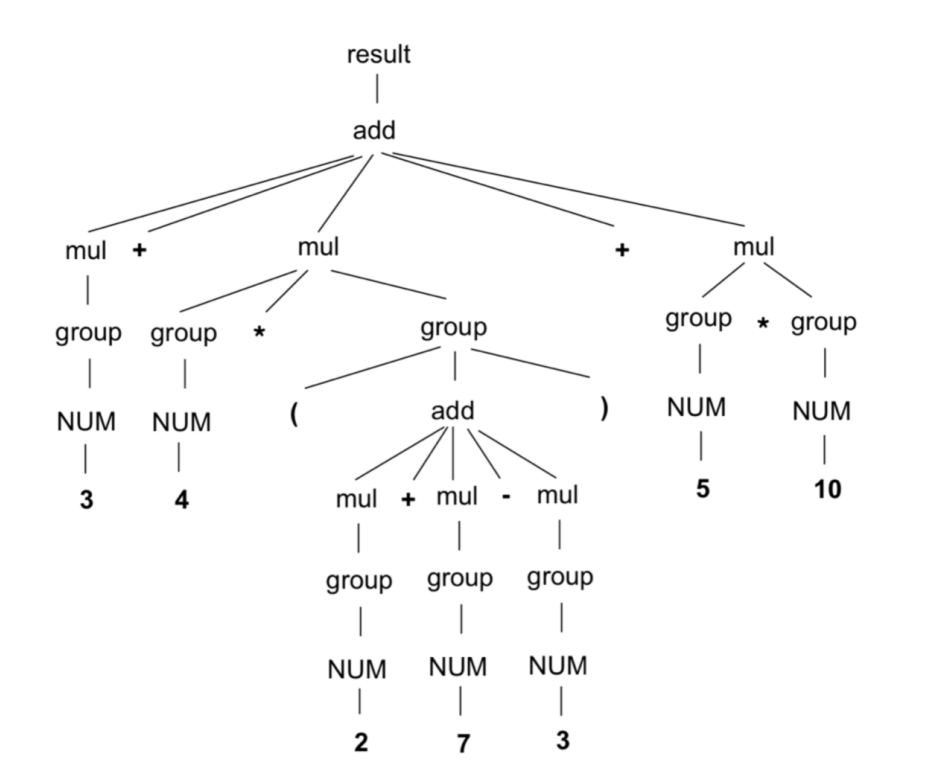
\includegraphics[width=15cm]{Images/ASP treea.png}
    \caption{Результат синтаксического анализав виде абстрактного синтаксического дерева – AST }
    \label{fig:2}
\end{figure}


